\vspace{-.15in}\section{Research Plan and Methodology}
\label{sec:rep}\vspace{-.075in}

\xxx strenghens the reliability of datacenter computing with a holistic 
methodology. This section first proposes \falcon (\S\ref{sec:protocol}), a fast 
and scalable consensus protocol, it then leverages \falcon to build a scheduler 
(\S\ref{sec:scheduler}) and a VM replication infrastructure (\S\ref{sec:vm}) to 
improve the availability of applications running in these infrastructures. 
Finally, this section describes research plan (\S\ref{sec:plan}).
% The first two objectives include preliminary results. 

\vspace{-.15in}\subsection{Objective 1: Building Fast, Scalable Consensus via
RDMA}\label{sec:protocol}\vspace{-.075in}

This section describes a performance problem (\S\ref{sec:latency-problem}) in 
existing \paxos procotols and presents \falcon (\S\ref{sec:falcon}), a 
fast, scalable \paxos protocol by leveraging RDMA.

\vspace{-.15in}
\subsubsection{Problem: Consensus latency of existing \paxos 
protocols scale poorly} 
\label{sec:latency-problem}\vspace{-.075in}

% P1: as mentioned in background, a key reason is thread interleavings, 
% so we need to reason about the general patterns we have. Or we say our 
% methodology is just like pattern matching.
% Traditional \paxos protocols incur high consensus latency because they go 
% through OS kernels and software TCP/IP layers. In this 
% section, \S\ref{sec:problem} analyzes this latency problem and its poor 
% scalability in detail, and then presents our new RDMA-based \paxos 
% protocol called \falcon (\S\ref{sec:falcon}).

% First, mainly introduce the problems in traditional protocols.
% Due to the strong fault-tolerance of \paxos, it is widely served in many 
% systems. For instance, Scatter~\cite{scatter:sosp11} runs 8$\sim$12 replicas in 
% each \paxos group to order client requests, and it lets replicas respond 
% requests in parallel. A bigger group size will improve Scatter throughput. 
% Moreover, recent state machine replication (SMR) 
% systems~\cite{eve:osdi12,rex:eurosys14,crane:sosp15} use \paxos to greatly 
% improve the availability of
% general server programs.

Despite the wide deployments of \paxos (\S\ref{sec:consensus}), its high 
consensus latency makes many software systems suffer. For efficiency, \paxos 
typically assigns one replica as the leader to invoke consensus requests, and 
the other replicas as backups to simply agree on requests. To agree on an 
input, at least one message round-trip is required between the leader and a 
backup. A round-trip causes big latency (hundreds of \us) as it goes through 
TCP/IP layers such as software network stack and OS kernel. This latency may 
be acceptable for leader election~\cite{chubby:osdi,zookeeper} or heavyweight 
transactions~\cite{crane:sosp15,eve:osdi12}, but undesirable for
key-value store applications~\cite{redis,memcached}.

As replica group size increases, \paxos consensus latency often increases
drastically~\cite{scatter:sosp11} due to the linearly increasing number of 
consensus messages. One common approach to improve \paxos scalability is 
leveraging parallel techniques such as multithreading~\cite{zookeeper, 
spaxos:srds12} or asynchronous IO~\cite{crane:sosp15, libpaxos}. However, the 
high TCP/IP round-trip latency still exists, and synchronizations in these 
techniques frequently invoke expensive OS events such as context switches.

Our preliminary study (Figure~\ref{fig:scalability}) ran four \paxos-like 
protocols~\cite{zookeeper, spaxos:srds12, crane:sosp15, libpaxos} on 40Gbps 
network with only one client sending consensus requests. We found that, when 
replica group size increased from 3 to 9, the consensus latency of three 
protocols increased by \tradlatencyincreaselow to 
\tradlatencyincreasehigh, and \systemcostlow to \systemcosthigh of the increase 
was in OS kernel.

% Second, briefly mention the problem in DARE. and its scalability bottleneck.
As the increasing popularity of RDMA, it becomes a promising 
approach to address the \paxos performance problem. However, fully exploiting 
RDMA speed in software systems is widely considered challenging by 
the community~\cite{pilaf:usenix14,herd:sigcomm14,
farm:sosp15,dare:hpdc15}. For instance, \dare~\cite{dare:hpdc15} presents a
two-round, RDMA-based \paxos protocol in a sole-leader manner: leader does all 
RDMA workloads and backups do nothing. \dare was fast with 3$\sim$5 
replicas. However, our study shows that, as replica group grows, \dare's 
sole-leader and two-round protocol incurred scalability bottlenecks: the 
consensus latency increased by \darescalability as the group growed by 35x (a 
linear increase, Figure~\ref{fig:scalability}).

\vspace{-.15in}\subsubsection{Falcon: a fast, scalable RDMA-based \paxos 
protocol} 
\label{sec:falcon}\vspace{-.075in}

Our key observation is that we should carefully separate RDMA workloads among
the leader and backups, especially in a scalability-sensitive context. 
Intuitively, we can let both leader and backups do RDMA writes directly on 
destination replicas' memory, and let all replicas poll their local memory to 
receive messages.

Although doing so will consume more CPU resources than a sole-leader 
protocol~\cite{dare:hpdc15}, it has three major benefits. First, the leader 
has less workloads. Second, both leader and backups participate in consensus, 
which makes it possible to reach consensus with only one 
round~\cite{paxos:practical}. Third, all replicas can just receive consensus 
messages on their bare, local memory. An analogy is threads receiving other 
threads' data via bare memory, a fast and scalable computation pattern.

We present \falcon,\footnote{We name our protocol after
falcon, one of the fastest birds.} a new RDMA-based \paxos protocol and its
runtime system. In \xxx, all replicas directly write to destination
replicas' memory and poll messages from local memory to receive messages, and 
our runtime system handles other technical challenges such as cheecking message 
delivery and recovering replica failures.

To support general, unmodified applications, \falcon stems from our preliminary 
general protocol, \crane~\cite{crane:sosp15}. Within \falcon, an application 
runs as is. \falcon automatically deploys this program on replicas, intercepts 
inputs from an application's inbound socket calls (\eg, \recv) with a Linux 
technique called LD\_PRELOAD, and invokes its consensus protocol to enforce same 
application inputs across replicas. Figure~\ref{fig:falcon-arch} shows 
\falcon's architecture with four key components: our consensus protocol for 
enforcing same inputs across replicas, an output checker for checking network 
outputs across replicas with our same protocol, an in-memory consensus 
log, and a guard process that handles checkpointing and recovering application 
execute states.

Figure~\ref{fig:falcon-protocol} shows \falcon's consensus protocol in normal 
case. The leader first executes the actual inbound socket call to get the 
actual inputs (\textbf{L1}, not shown), it then invokes consensus across 
replicas. All solid arrows (\textbf{L3} and \textbf{B2}) are ultra-fast RDMA 
direct writes to remote replicas' memory. All replicas poll from their own bare 
memory to receive consensus messages. To handle replica failures, all replicas 
persitently log inputs to local storage. For these writes, because the sending 
replicas only need to copy the sent data to local RDMA network interface card 
and then the writes finish on local site, \falcon is scalable when more backup 
replicas are added.

% Three figures. First, falcon arch. Second, consensus protocol. Third, falcon 
% results compared to traditional ones and DARE.

\begin{figure}[!htb]
    \begin{minipage}{.4\textwidth}
        \vspace{-.2in}
        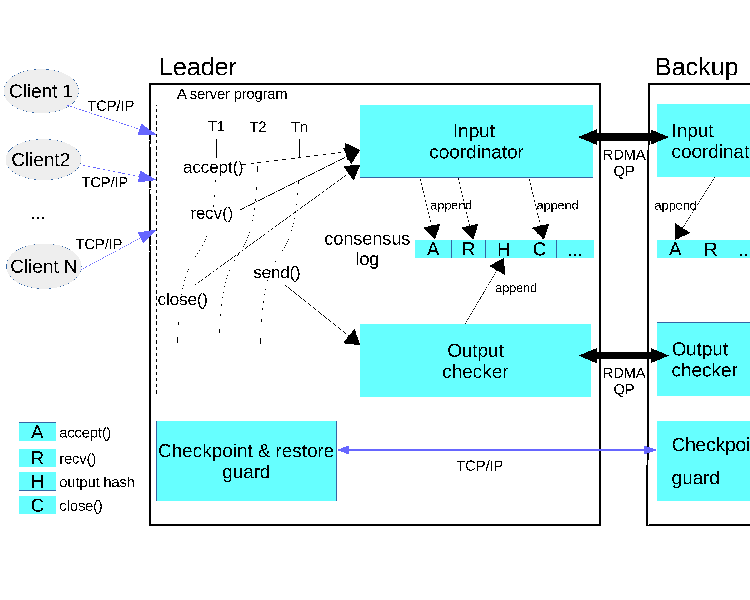
\includegraphics[width=0.34\textheight]{figures/arch.ps}
        \vspace{-.4in}         
        \caption{The \falcon architecture.}
        \label{fig:falcon-arch}
    \end{minipage}
    \begin{minipage}{0.4\textwidth}
        \vspace{-.2in}
        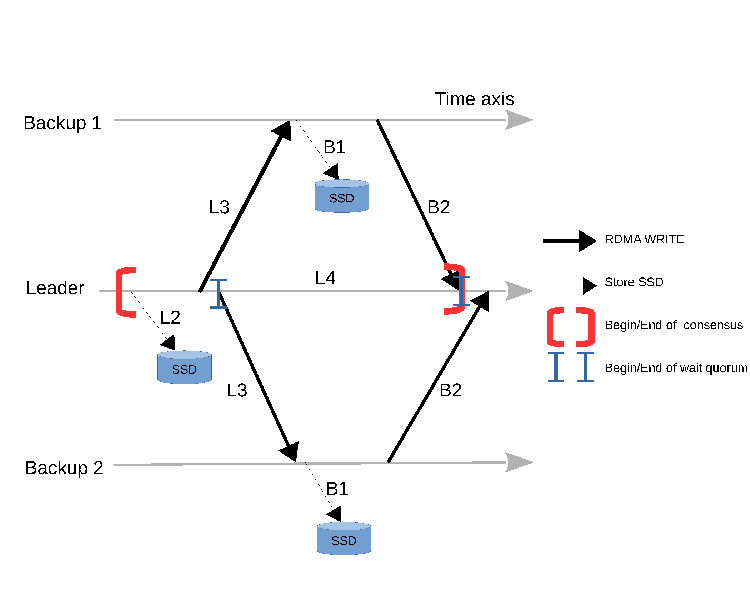
\includegraphics[width=0.34\textheight]{figures/consensus.ps}
        \vspace{-.4in}
        \caption{\falcon consensus protocol.}
        \label{fig:falcon-protocol}
    \end{minipage}
\end{figure}

\para{Primilinary results.} Our preliminary results include two steps. First, 
to justify whether such a general, socket-intercepting protocol can support 
general applications, we have developed \crane~\cite{crane:sosp15}. \crane was 
able to support five widely used server applications (\eg, \mysql) without 
modifying them. Second, we built \falcon, a much faster and more scalable 
version of \crane, by leveraging RDMA. Figure shoes \falcon performance with 
existing consensus protocols. \falcon was one order of magnitude faster latency 
than the literature. \falcon's consensus latency outperforms 4 popular \paxos 
protocols by \comptradlow to \comptradhigh on 3 to 9 replicas. \falcon is 
faster than \dare by up to \fasterDARE. When changing the replica group size 
from 3 to 105 (a 35x increase), \falcon's consensus latency increases merely 
from \xxxlatencythree \us to \xxxlatencyonezerofive \us (a \xxxscalability, 
sub-linear increase).
% Crane. Falcon. Say Crane is first version. Falcon 
% totally subsumes Crane. Falcon also has initial results.

\begin{figure}[!htb]
\centering
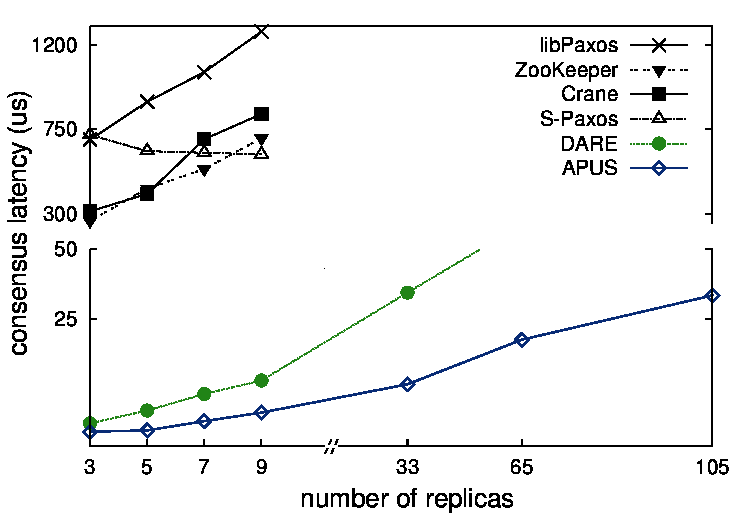
\includegraphics[width=0.34\textheight]{figures/traditional_paxos_latency.ps}
        \vspace{-.2in}
        \caption{Consensus latency of six \paxos protocols. \falcon is fastest 
and scales the best.}
        \label{fig:scalability}
\end{figure}

\para{Future work.} Since \falcon is the keystone of our objectives, this 
proposal plans to further study and improve its practicality in three aspects: 
(1) study its performance and potential bottlenecks on thousands of replicas, 
and propose new solutions; (2) study its protocol robustness on failure 
scenarios, including leader election and adding/removing replicas; and (3) 
evaluate its generality on more latency-critical applications. 

\vspace{-.15in}\subsection{Objective 2: Integrating \falcon with datacenter 
schedulers}\label{sec:scheduler}\vspace{-.075in}

Indeed, many existing schedulers have adopted \paxos to improve availability 
for themselves. Typically, they use \paxos to run multiple copies of their 
controllers, which works on scheduling computation jobs with resources. In 
normal case, only one leading controller does the real work, and the others 
standby to cope with the leader's failure. Unfortnately, most applications 
running by these schedulers have not been made highly-available (although minor 
applications implement a replication 
approach~\cite{mapreduce,dolly:nsdi13}).

A naive approach to achieve high application availability could be implementing 
a \paxos within each application. However, this approach has two major issues. 
First, \paxos is notoriously difficult to 
understand~\cite{raft:usenix14,paxos:simple}, implement~\cite{paxos:practical, 
paxos:live}, or test~\cite{modist:nsdi09,demeter:sosp11}, thus developing a 
\paxos protocol for each application is widely considered a 
nightmare~\cite{modist:nsdi09,demeter:sosp11,paxos:live} for application 
developers.

The second issue is, the scheduler may defeat \paxos due to unawareness of the 
application's \paxos replication logic. For instance, if an application submits 
multiple copies of the same computation job to the scheduler, the scheduler may 
incorrectly schedule several copies on the same computer (it should schedule 
each copy on different computers to achieve \paxos fault-tolerance).

\vspace{-.15in}\subsubsection{\tripod: the fault-tolerant scheduler 
architecture} 
\label{sec:scheduler-arch}\vspace{-.075in}

% ,\footnote{We name our system after 
% the ancient Chinese three-legged tripod, a reliable, multi-purpose container.}
This section proposes the design of \tripod, a scheduler infrastructure that 
automatically provides high-availability to general applications. \tripod 
is integrated with a widely used scheduler \mesos~\cite{mesos:nsdi11} and 
\falcon (\textbf{Objective 1}). To avoid the two aforementioned issues 
(\S\ref{sec:scheduler}), \tripod chooses 
to integrate \paxos in a scheduler, not in applications. To achieve high
application availability, unlike existing schedulers which let only one 
controller schedule jobs, \tripod runs replicas of the same job using replicas 
of controllers: after controllers agree on a new job with \falcon, \tripod lets 
each controller independently schedule an copy of this job.

Doing so has three benefits. First, \tripod's \paxos acts as a single, general 
fault-tolerance service to applications. We can just leverage existing 
verification tools~\cite{modist:nsdi09,demeter:sosp11} to make sure that our 
\falcon protocol is robust and correct, and then we can benefit many 
applications. Second, application developers can now just focus on their own 
application logic, greatly saving development time and money. Third, now 
\tripod's own scheduler can handle the replication logic and do careful, 
replication-aware scheduling for jobs  (\S\ref{sec:workflow}). 


% To 
% ahieve application fault-tolerance, 



% In an implementation level, \tripod integrates \mesos~\cite{mesos:nsdi11}, a 
% widely used cluster management system, with a new RDMA-enabled \paxos 
% protocol~\cite{falcon:github}. Compared to a prior RDMA-enabled \paxos 
% protocol~\cite{dare:hpdc15}, our new protocol can support general programs 
% transparently without modifications.

Figure~\ref{fig:scheduler-arch} depicts \tripod's architecture, and its key 
components are shaded (and in blue). To illustrate how \tripod works in an 
application perspective, this figure shows two applications, Hadoop and MPI. 
Each application has a \emph{replica strength} (\v{R}) to denote the level of 
fault-tolerance it demands. This value is either 1 or equals the number of 
replicas of controllers in \tripod.

By default, each application has \v{\v{R}=1}, which means that this application 
does not need replication. For such a default setting, \tripod runs the job as 
is without replication, like a typical cluster management system (\eg, Mesos).

In this figure, Hadoop's \v{R} is 3, which means that it wants to replicate 
each of its job with three copies for high-availability. Suppose Hadoop 
submits two jobs to the leader controller, each has different shapes (triangle 
or hexagon). The leader controller then invokes a consensus on each job across 
controllers. Once a consensus is reached, each controller assigns the same job 
on different slave machines. The leader controller directly returns its 
computation result to the Hadoop scheduler. Standby controllers ignore the 
results unless the same mechanism is triggered.
%  unless a tail-tolerance mechanism is triggered 
% (\S\ref{sec:workflow})

\begin{figure}[!htb]
    \begin{minipage}{.49\textwidth}
        \vspace{-.2in}
        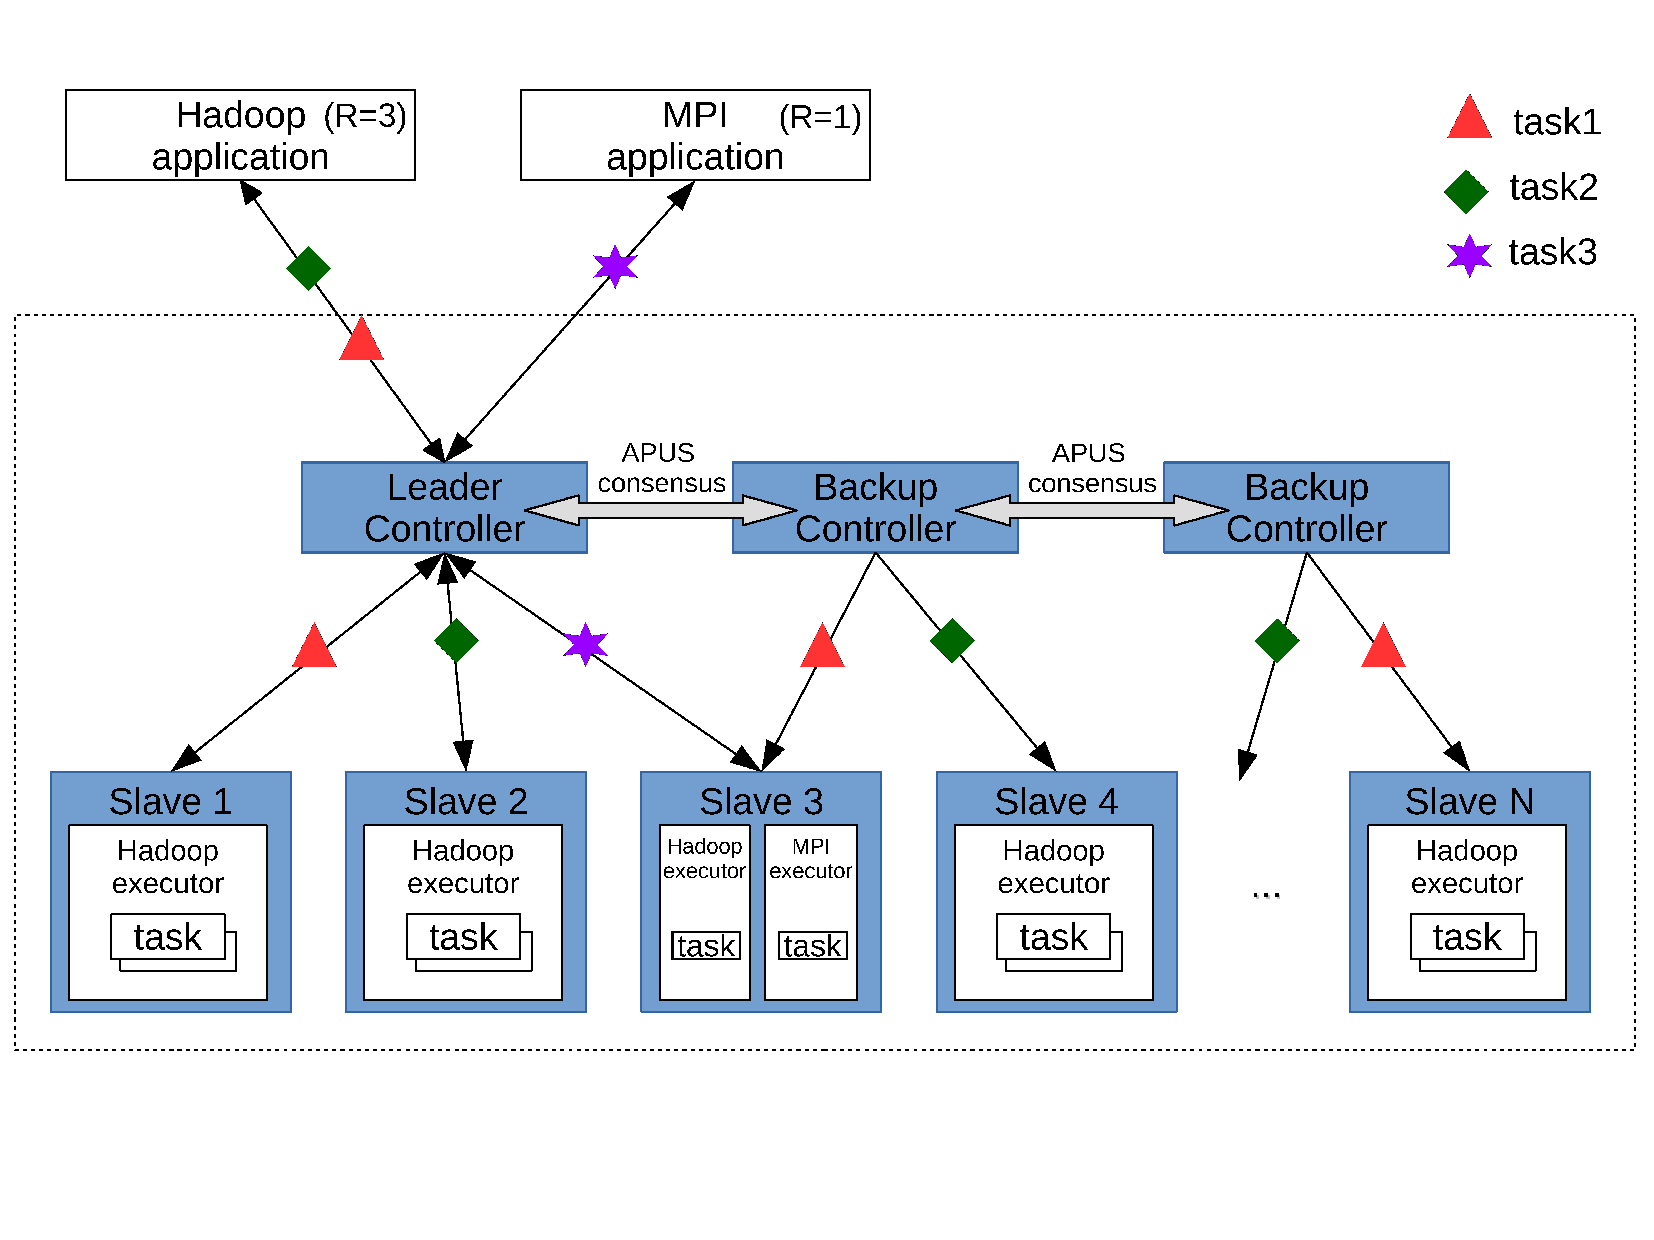
\includegraphics[width=0.34\textheight]{figures/scheduler_arch.ps}
        \vspace{-.3in}
        \caption{Fault-tolerant scheduler.}
        \label{fig:scheduler-arch}
    \end{minipage}
    \begin{minipage}{0.51\textwidth}
        \vspace{-.2in}
        
\includegraphics[width=0.34\textheight]{figures/scheduler_flow.ps}
        \vspace{-.3in}
        \caption{Workflow.}
        \label{fig:scheduler-workflow}
    \end{minipage}
\end{figure}

\vspace{-.15in}\subsubsection{Replication-aware resource allocation workflow}
\label{sec:workflow}\vspace{-.075in}

Figure~\ref{fig:scheduler-workflow} shows \tripod's workflow on scheduling jobs 
with four steps. This workflow is similar to that in Mesos except the second 
and fourth steps. These two steps \tripod abstract away the replication logic 
in its resource offers and allocations from the application. An application runs 
as if \xxx does not replicate any of its jobs, and \tripod transparently 
handles all the replication logic.

In the first step, slave machines periodically report their available computing 
resources (\eg, CPU cores and memory) to the leader controller. In the second 
step, instead of offering the available resources aggregated from slave 
machines, \tripod divides the amount of resources by each application's \v{R} 
value and then sends a resource offer to the application. The goal is to 
reserve enough resources for \tripod to replicate a job with \v{R} copies.

In the third step, an application scheduler submits jobs to the leader 
controller. The leader controller then invokes a consensus on this job by 
carrying the resource offer made to the application.

Once a majority of controllers agrees on executing this job, each controller 
does the fourth step. It schedules this job on an available slave machine 
according to the resource offer. To prevent controllers putting the same job on 
the same slave machine, the leader controller first makes an assignment on 
which controller should run this job on which slave machine, it then carries 
this assignment in its consensus request. Once a consensus on this job is 
reached, each controller follows this assignment.

% Two figures: one is TRIPOD arch. The other is TRIPOD results from the workshop 
% paper. Figure~\ref{fig:scheduler-arch} and Figure~\ref{fig:scheduler-workflow} 
% and Figure~\ref{fig:scheduler-latency}.


\para{Availability v.s. resource consumption.} \tripod is designed to make a
mission-critical applicaion highly avaialble by leveraging \v{R} times of 
resources than the application's native, unreplicated execution. We deemed this 
extra resource consumption reasoanble for two reasons.

First, a major trend is that an application runs on more and more 
computers, thus minor computer failures tend to happen more likely. Such 
failures may turn down the entire application and cause if the failure computer 
runs a critical computation. For instance, Both NYSE and Nasdaq have experienced 
outage of their whole site~\cite{nyse:halt} or specific IPO 
events~\cite{facebook:ipo:delay} due to minor machine errors. 
In addition, social-networking applications like Facebook has 
strong fault-tolerance requirements, because minor machine failures have turned 
down the whole Facebook site for several times in the last few 
years~\cite{facebook:outage}, costing huge money lost. 

Second, it is already a common practice to replicate critical computations by 
using \v{R} times of resources, and doing so can improve both availability and 
performance. For instance, Scatter~\cite{scatter:sosp11} runs 8$\sim$12 
replicas in a \paxos group to order client requests, and it lets replicas reply 
requests in parallel. A bigger group size will improve Scatter throughput. 
Moreover, several recent replication 
systems~\cite{eve:osdi12,rex:eurosys14,crane:sosp15} 
improve the availability of general server applications (\eg, 
\mysql~\cite{mysql}) by replicating them.

% Therefore, \tripod's design favors more on availability and performance 
% (low consensus latency). It's design tends to use \v{R} times of resources 
% compared to traditional applications. We argue that this extra resource 
% utilizations are acceptable for critical applications, because if they have 
% high 
% demand on availability and response times, they can often tolerate costs on 
% computing resources (\eg, trading and medical platforms).



\para{Primilinary results.} We built a preliminary \tripod propotype, 
published in [APSys '16]. To evaluate a typical social-networking application, 
we ran \tripod with \memcached~\cite{memcached}, a popular key-value store used 
by Twitter and financial platforms~\cite{nosql:finance}. Compared to 
\memcached's unreplicated execution, \tripod incurred merely a \tputoverhead 
overhead in throughput and \latencyoverhead in response time.
% This protocol was 40.1X faster than \zookeeper, a traditional replication
% protocol~\cite{calvin:sigmod12} which runs on TCP/IP.

% Disable the figure for now. Not much information.
% \begin{figure}[!htb]
% \centering
% 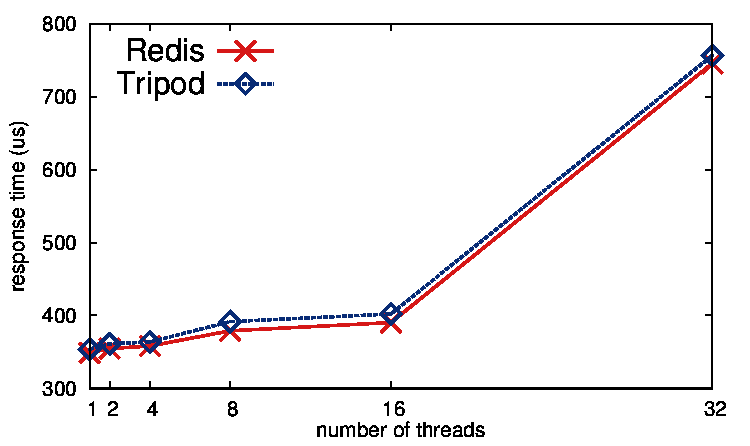
\includegraphics[width=0.34\textheight]{figures/scheduler_latency.ps}
%         \vspace{0.1in}
%         \caption{Performance overhead of scheduler.}
%         \label{fig:scheduler-latency}
% \end{figure}

\para{Future work.} Our \tripod development will go along two directions. 
First, currently our replication and resource allocation workflow is tied with 
\mesos. We will study other popular schedulers and summarize their 
resource allocation workflow patterns, and we will develop a general, 
scheduler-agnostic workflow. Second, we will study new differential replication 
schemes, so that we can flexibly assign different \v{R} values to different 
compnents of an appilcation, getting both satisfiable availability and optimal 
resource consumption.

\vspace{-.15in}\subsection{Objective 3: Strenghening VM to improve application 
availability}\label{sec:vm}\vspace{-.075in}




Virtual machines (VM) infrastructures (\eg, Amazon EC2~\cite{amazon:vpc} and 
OpenStack~\cite{openstack}) are widely deployed in datacenters and clouds 
because they can provide a virtualized abstraction of computing resources to 
different applications and enforce strong utiilization isolation and security. 

As mentioned in related work (\S\ref{sec:others-work}), two approaches, 
primary-backup and live migration, exist for improving VM fault-tolerance, 
resource utilization, and energy saving. Both these approaches face problems on 
substantial application down time (\eg, 8 seconds in a live migration system 
vMotion~\cite{vmotion:atc05}) and network bandwidth. The downtime hurts 
application availability even if there is no replica failure. The bandwidth 
consumption often aggravates resource burdens because these approaches are often 
invoked when resources are tight.

A main reason that causes these two problems is that these approaches have only 
one actual execution of an application. Therefore, once execution states is 
required to transfered to a remote computer, the local execution has to be 
disturbed.


% Therefore
% Mainly introduce EC2, Openstak. VM only.

% Briefly introduce VM fault-tolerance techniques. Primary-backup. Remus. 
% Hypervisor replication (old paper). FaRM.
% 
% Talk about migration. It is similar to primary-backup, but mainly for load 
% balance, not to overcome failures. Main approach is live migration that aims to 
% reduce application down time. VMotion.

% However, there is still substantial down time and resource consumption. E.g., 
% vMotion, for memory intensive applications, the down time can be up to 30 
% seconds. As migration tends to invoke frequently for load balancing, 
% consolidation, energy saving, this downtime may incur big money lost for cloud 
% deployers.

% When doing migration, both the local computer and the migration destination 
% computer incur big resource consumption. This is contraditive to the motivation 
% of migration: reduing computer loads on the local computer.

\vspace{-.15in}\subsubsection{Forming an eco-system with VM and \falcon} 
\label{sec:vm-arch}\vspace{-.075in}

\begin{figure}[!htb]
\centering
\vspace{-.2in}
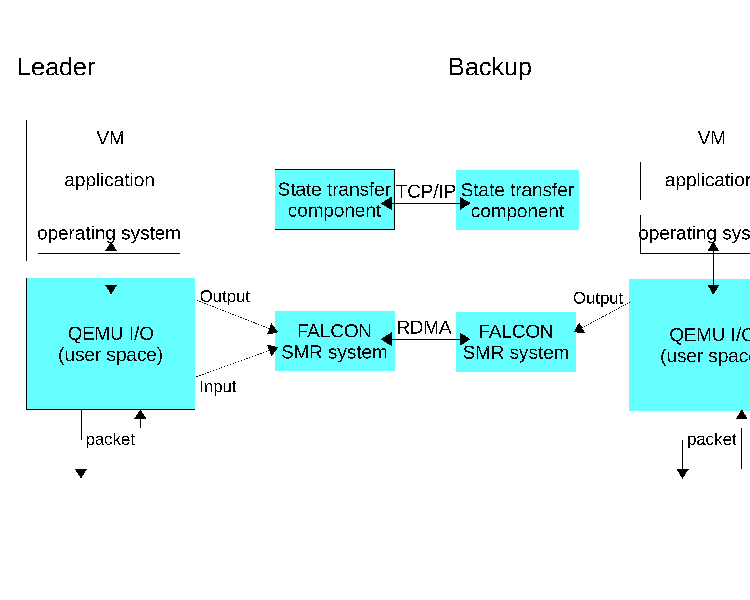
\includegraphics[width=0.34\textheight]{figures/vm_arch.ps}
        \vspace{-.3in}
        \caption{Performance overhead of scheduler. Our key components are 
shaded (and in blue color).}
        \label{fig:vm-arch}
\end{figure}

Fortunately, \paxos-based replication can construct multiple, equivalent 
executions for the same application, thanking to its robustness and 
consistency. To ensure high application avaialbility, we can just run \paxos to 
make replicas of VMs see the same sequence of inputs, and doing so is feasible 
because many VM architectures have input interception layers by default.

We make \falcon and VM form a mutual-beneficial eco-system. In this eco-system, 
VM provides a hypervisor layer to automatically capture incoming inputs and 
application execution state changes for \falcon, and \falcon benefits a VM by: 
(1) improving avaialbility of applications running in this VM, and (2) greatly 
improving application downtime and bandwidth consumption for the VM's live 
migration.

Figure~\ref{fig:vm-arch} shows the architecture of the eco-system. To provide 
the same fault-tolerance guarantee with primary-backup, a typical replication 
factor of this eco-system is \v{R=3}. This eco-system chooses KVM~\cite{kvm} 
due to two main reasons. First, KVM is an open source hypervisor carried in 
Linux. Second, it provides \v{tap\_send()}, an input capturing API at its QEMU 
component running at user space. Compared to other types of hypervisors, this 
API enables \falcon to coordinate inputs with RDMA, because currently RDMA only 
supports user space.

A key benefit of such a \paxos-based VM replication over primary-backup is that 
its leadership is strongly consistent (through a majority aggrement, which 
primary-backup lacks), and it saves the bandwidth consumption for transfering 
application execution states in primary-backup.

% Describe the infrastructure. Take Ning's figure. Hypervisor. tap\_send().

\vspace{-.15in}\subsubsection{\paxos-based Live Migration} 
\label{sec:vm-migration}\vspace{-.075in}

Interestingly, this replication ability not only provides high 
availability for fault-tolerance (suitable for the primary-backup scenario), 
but can also greatly save resource consumption if fault-tolerence is not a 
major concern (suitable for the live migration scenario). Consider the live 
migration scenario, \paxos backups can only agree on inputs without actually 
executing them, then the overall application execution consumes almost same 
resources as the unreplicated one. A backup now can just absorb occasional, 
periodical application checkpoints from the leader when the leader replica is 
idle, and catches up with the leader when a migration destination is decided on 
this backup.

% We propose our own replication approach. The non-leader only agree on new 
% inputs, they can opt to execute requests or absorb periodic checkpoints.
Leveraging this idea, we propose a fast, network bandwidth-friendly live 
migration approach called ``\paxos-based live migration". A key benefit of this 
approach is that, now migration does not require transfering all execution 
states of application, but only tranferfing the \paxos leadership (almost as 
fast as \paxos consensus latency) to a destination backup which has idle 
resources. To increase the chance on finding a proper destination, we can 
leverage \falcon's high availability to run many backups within a datacenter.

% This approach is othorgnal to the VM replication. 
This \paxos-based live migration approach contains four steps. First, in 
normal case, the current computing instance (the leader) just agrees on 
incoming inputs with backups using \falcon. A set of backups run on hightly 
loaded computers and agree on inputs (also record the inputs persistantly). 

Second, the leader does a periodical checkpoint when it's idle (no incoming 
requests), and sends the checkpoint to the backups. The backups only keeps 
the latest checkpoint and discards prior ones.

Third, when the VM invokes a migration on the leader computer, it uses a 
standard migration mechanism to determine which backup should be the migration 
destination (the next leader). Then, the destination extracts the lastest
checkpoint on local computer, restores the application state, and then catches 
up with the leader with executing the recorded but not executed inputs.

Fourth, we invoke a \falcon protocol level operation: migration the 
leadership, which is similar to a traditional \paxos leader election 
process~\cite{paxos:practical}, but we just explicitly decide the destination 
computer as the new leader. \falcon's protocol handles various failure 
scenarios (\eg, the destination computer crashes during the migration) as its 
\paxos nature.

% TBD: mention the leader election latency in Objective 2.
% Analysis: this approach incurs almost zero time and resource for a few reasons. 
% First, the leadership migration is fast (tens of micro seconds). Second, no 
% frequent execution state transfer during the migration time, only at the 
% leader's idle time. Third, robust to various scenarios (\eg, destination fails 
% during the migration), thanking to \paxos.

\para{Future work}. We plan to fully implement the eco-system, including both 
the replication architecture (\S\ref{sec:vm-arch}) and the novel live 
migration approach (\S\ref{sec:vm-migration}). We will compare the 
performance overhead of our replication approach with existing open-source VM 
infrastructure (\eg, OpenStack). We will also compare the performance of our 
migration approach with existing live migration approaches (\eg, vMotion).


% % TBD: need a new replication approach name.
% \vspace{-.15in}\subsubsection{Idea I: Hybrid Replication} 
% \label{sec:defense-arch}\vspace{-.075in}
% 
% TBD.

\vspace{-.15in}\subsection{Research Plan} \label{sec:plan}\vspace{-.075in}

This project will require two PhD students S1 and S2 to work for 
three years. In the first year, S1 will design and fully implement the \falcon 
protocol (part of \textbf{Objective~1}), and S2 will evaluate its performance 
and robustness on various real-world storage applications (part of 
\textbf{Objective~2}). In the second year, S1 will 
integrate \falcon to a scheduler \mesos (part of \textbf{Objective~2}), and S2 
will make \falcon and KVM form an eco-system (part of \textbf{Objective~3}). In 
the third year, S1 and S2 will respectively study the efficacy of their systems 
built Object 2 and Object 3 with real-world applications, including big data 
applications.
% Both students will 
% involve theoretical methods, implement real software systems, and 
% perform real-world study.
% The PI will supervise the students by providing 
% advice concerning both theoretical and systems implementation levels.


